%!TEX root = ../Main.tex
\section{Clustering with filters}
\label{clustering:s:Introduction}
% A collection-oriented programming model is ideal for expressing data-parallel computations, as it exposes the communication patterns to the compiler without requiring complicated loop analysis.
% It is essential, however, that the compiler combines these operations into a small number of efficient loops, as a naive translation leads to high memory traffic and poor performance.
% This is a well known problem, and techniques to fuse subsequent array operations together have been presented in~\cite{gill1993short, coutts2007stream, keller2010repa}, to name just a few.
% This type of fusion alone is not generally sufficient to minimise memory traffic.
% % : first, we often need to re-arrange the array operations and cluster those that iterate over the same structures.
% As shown in Megiddo~\cite{megiddo1998optimal} and Darte~\cite{darte2002contraction}, Integer Linear Programming can be used to find good clusterings.
% Unfortunately, they cannot handle operations like filter, where the output size differs from the input size.
% We present a technique that can handle both multi-loop fragments as well as size-altering operations. 

% To compile the clusters found by our clustering technique into sequential loops, we use data flow fusion~\cite{lippmeier2013data}.
% It improved on existing array fusion approaches~\cite{coutts2007stream, keller2010repa} as it guarantees fusion into a single loop for programs that operate on the same size input data and contain no fusion-preventing dependencies between operators. 
% Our clustering technique is also applicable to parallel loops.


% To compile collection-oriented array functional array programs, which play a particular important role in parallel programming, into efficient code, it is essential that we can compile the array operations to a small number of imperative loops. Data flow fusion~\cite{lippmeier2013data} addressed this problem by presenting a technique to compile a specific class of data flow programs into single, efficient imperative loops. It improved on existing related array fusion approaches (~\cite{coutts2007stream}, ~\cite{keller2010repa} as it 1) it fuses programs that use branching data flows where a produced array is consumed by several consumers, and 2) guarantees complete fusion into a single loop for all programs that operate on the same size input data and contain no fusion-preventing dependencies between operators. However, it can only fuse code fragments into one loop that produce a single output array. Approaches based on Integer Linear Programming (\cite{megiddo1998optimal} and Darte~\cite{darte2002contraction}) do not suffer from this shortcoming. On the other hand, they cannot handle operations like filter, which produce arrays whose size differs from the input arrays.  The technique we present in this paper can handle both multi-loop fragments as well as size-altering operations. 

To see the effect of clustering, consider the following array program:

\begin{haskell}
normalize2 :: Array Int -> (Array Int, Array Int)
normalize2 xs
 = let sum1 = fold   (+)  0   xs
       gts  = filter (>   0)  xs
       sum2 = fold   (+)  0   gts
       ys1  = map    (/ sum1) xs
       ys2  = map    (/ sum2) xs
   in (ys1, ys2)
\end{haskell}

The \Hs@normalize2@ function computes two sums: one of all the elements of \Hs@xs@, the other of only elements greater than zero.
The two maps then divide each element in the input \Hs@xs@ by \Hs/sum1/ and \Hs/sum2/, respectively.
Since we need to fully evalute the sums before we can start to execute either map, we need at least two separate passes over the input.
These folds are examples of \emph{fusion-preventing dependencies}, as fold must consume the entire input stream before it can produce its result, and this result is needed before the next stream operation can begin.
A fusion-preventing dependency between two combinators means that the two combinators must be assigned to different clusters.

\Cref{clustering:f:normalize2-clusterings} shows three cluster diagrams for \Hs@normalize2@, with each clustering produced by a different clustering algorithm.
A cluster diagram is an extended version of the dependency graphs we have already seen; we explain the details in \cref{clustering:s:CombinatorNormalForm}.
The leftmost diagram shows how we have to break this program up to execute each part, assuming we use the pull stream model from \cref{taxonomy/pull}.
With pull streams we cannot compute the sums or the maps concurrently, so we end up with four loops, denoted by dotted lines in the diagram; only the filter operation is combined with the subsequent fold.
If we wrote this program to use stream fusion \citep{coutts2007stream}, which is a form of pull-based shortcut fusion, we would end up with the same clustering.
% We benchmarked our process fusion against the Vector library earlier, in \cref{s:Benchmarks}.

\begin{figure}
\begin{center}
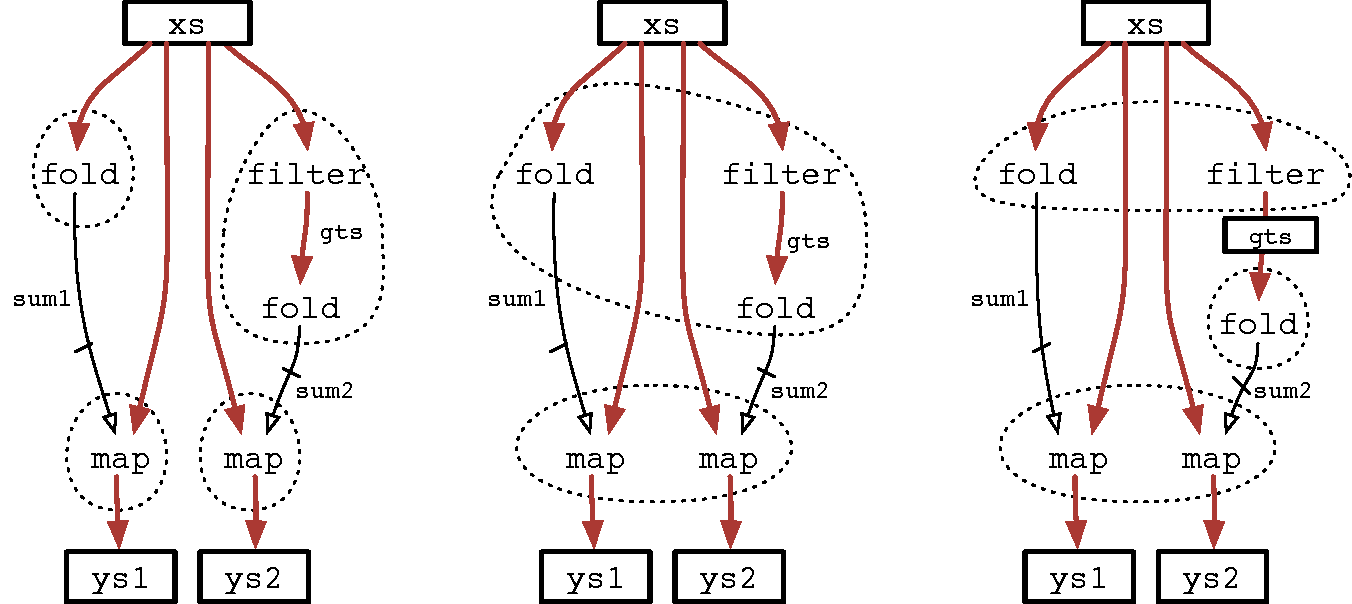
\includegraphics[scale=0.5]{copy/03-body/clustering/figures/ex1-compare.pdf}
\end{center}
\caption{Clusterings for \Hs/normalize2/: with pull streams; our system; best imperative system}
\label{clustering:f:normalize2-clusterings}
\end{figure}


The rightmost diagram in \cref{clustering:f:normalize2-clusterings} shows the clustering determined by the best existing ILP approach for imperative array-based loop fusion.
To obtain this clustering, we first implemented each combinator as a separate imperative loop, shown in \cref{figs/clustering/normalize2-c}.
Imperative clustering algorithms, such as \citet{megiddo1998optimal}, only cluster together loops of the same iteration size.
% The loop that performs the filter operation consumes the array \Hs/xs/, which has size \Hs/xs_length/, and produces the array \Hs/gts/, which has size \Hs/gts_length/.
In the imperative code, the loop that performs the fold over \Hs/gts/ has an iteration size of \Hs/gts_length/, while all the other loops have an iteration size of \Hs/xs_length/.
The final value of \Hs/gts_length/ is not known until the loop that performs the filter completes, so there is a fusion-preventing dependency between the loop that performs the filter and the loop that performs the fold over \Hs/gts/, as well as having different iteration sizes.
The low-level imperative details obscure the high-level meaning of the program, and complicate fusing the filter operation with the subsequent fold.
% The imperative clustering combines the \Hs@sum1@ fold and \Hs@gts@ filter into one loop, as well as combining the two map operations.
% The imperative clustering combines the \Hs@sum1@ fold and \Hs@gts@ filter into one loop, as well as combining the two map operations.
% , but requires an extra loop for the fold operation which consumes the filter output, since it cannot fuse filter operations.

\begin{listing-c}[float,label=figs/clustering/normalize2-c,caption=Unfused imperative implementation of \Hs/normalize2/]
void normalize2(int* xs, int xs_length, int* out_ys1, int* out_ys2)
{
    // sum1 = fold (+) 0 xs
    int sum1 = 0;
    for (int i = 0; i != xs_length; ++i) {
        sum1 += xs[i];
    }

    // gts = filter ($>$ 0) xs
    int* gts = malloc(sizeof(int) * xs_length);
    int gts_length = 0;
    for (int i = 0; i != xs_length; ++i) {
        if (xs[i] > 0) {
            gts[gts_length] = xs[i];
            gts_length += 1;
        }
    }

    // sum2 = fold (+) 0 gts
    int sum2 = 0;
    for (int i = 0; i != gts_length; ++i) {
        sum2 += gts[i];
    }
    free(gts);

    // ys1 = map (/ sum1) xs
    for (int i = 0; i != xs_length; ++i) {
        out_ys1[i] = xs[i] / sum1;
    }

    // ys2 = map (/ sum2) xs
    for (int i = 0; i != xs_length; ++i) {
        out_ys2[i] = xs[i] / sum2;
    }
}
\end{listing-c}

Our approach, shown in the middle of \cref{clustering:f:normalize2-clusterings}, produces the optimal clustering in this case: one loop for the filter and folds, another for the maps.
For this example, we could execute each cluster as either push streams (\cref{taxonomy/push}) or as a process network fused by process fusion (\cref{chapter:process:processes}).
In general, a single cluster produced by our algorithm may contain combinators with multiple inputs as well as multiple outputs, so we execute each cluster as a fused process network.

% Data flow fusion~\cite{lippmeier2013data} is a technique to compile a specific class of data flow programs into single, efficient imperative loops. This process of ``compilation'' is equivalent to performing array fusion on a combinator based functional array program, as per related work on stream fusion~\cite{coutts2007stream} and delayed arrays~\cite{keller2010repa}. The key benefits of data flow fusion over this prior work are: 1) it fuses programs that use branching data flows where a produced array is consumed by several consumers, and 2) complete fusion into a single loop is guaranteed for all programs that operate on the same size input data, and contain no fusion-preventing dependencies between operators. This process of ``compilation'' is equivalent to performing array fusion on a combinator based functional array program, as per related work on stream fusion~\cite{coutts2007stream} and delayed arrays~\cite{keller2010repa}. The key benefits of data flow fusion over this prior work are: 1) it fuses programs that use branching data flows where a produced array is consumed by several consumers, and 2) complete fusion into a single loop is guaranteed for all programs that operate on the same size input data, and contain no fusion-preventing dependencies between operators.

% Fusion-preventing dependencies express the fact that some operators simply must wait for others to complete before they can produce their own output. For example, in the following:
% \begin{code}
%   normalize :: Array Int -> Array Int
%   normalize xs = let sum = fold (+) 0 xs
%                  in  map (/ sum) xs
% \end{code}

% If we wish to divide every element of an array by the sum of all elements, then it seems we are forever destined to compute the result using at least two loops: one to determine the sum, and one to divide the elements. The evaluation of @fold@ demands all elements of its source array, and we cannot produce any elements of the result array until we know the value of @sum@. 

% However, many programs \emph{do} contain opportunities for fusion, if we only knew which opportunities to take. The following example offers \emph{several} unique, but mutually exclusive approaches to fusion. \Cref{clustering:f:normalize2-clusterings} on the next page shows some of the possibilities.
% \begin{code}
%  normalize2 :: Array Int -> (Array Int, Array Int)
%  normalize2 xs
%   = let sum1 = fold   (+)  0   xs
%         gts  = filter (> 0)    xs
%         sum2 = fold   (+)  0   gts
%         ys1  = map    (/ sum1) xs
%         ys2  = map    (/ sum2) xs
%     in (ys1, ys2)
% \end{code}

% In \cref{clustering:f:normalize2-clusterings}, the dotted lines show possible clusterings of operators. Stream fusion implicitly choses the solution on the left as its compilation process cannot fuse a produced array into multiple consumers. The best existing ILP approach will chose the solution on the right as it cannot cluster operators that consume arrays of different sizes. Our system choses the solution in the middle, which is also optimal for this example. 

% NOTE: This set of bullets needs to fit on the first page, without spilling to the second.

% We must also decide which clustering is the `best' or most optimal. One obvious criterion for this is the minimum number of loops, but there may even be multiple clusterings with the minimum number of loops. In this case, the number of required manifest arrays must also be taken into account. 

% As real programs contain tens or hundreds of individual operators, performing an exhaustive search for an optimal clustering is not feasible, and greedy algorithms tend to produce poor solutions. 

